% =====================================================================
%  Final report, 02805 Social Graphs and Interactions (DTU)
%  PNAS research-article template (pnas-new.cls v1.47).
%
%  Course rules (week 8):
%   - at most 6 pages INCLUDING figures and references
%   - Abstract, Significance, Introduction, Results, Discussion,
%     Methods, References, specific author contributions
%   - three good figures beat eight; every caption says what is
%     plotted, what it is compared against, and what to see
%
%  Build: `make` in this folder (or see report/README.md).
%  Text lives in sections/*.tex, one file per section, so that we
%  can edit in parallel without merge conflicts.
% =====================================================================
\documentclass[9pt,twocolumn,twoside]{pnas-new}

% Line numbers in the margins help reviewers point at a line.
% true = numbered, as in the course template; false = clean preview.
\newif\ifshowlinenumbers
\showlinenumberstrue

\articletype{Social Sciences}  % classification shown on top of page 1

\templatetype{pnasresearcharticle}

% Local builds use Tectonic (XeTeX), which has no Type 1 Helvetica.
% TeX Gyre Heros is a Helvetica clone, so the PDF matches Overleaf
% (pdfLaTeX), where this block is skipped.
\ifxetex
  \usepackage{fontspec}
  \setsansfont{texgyreheros}[
    Extension=.otf, UprightFont=*-regular, BoldFont=*-bold,
    ItalicFont=*-italic, BoldItalicFont=*-bolditalic]
\fi

\ifshowlinenumbers\else
  \makeatletter
  \def\PNAS@mk@linecount{\savebox{\PNAS@linecount@bx}{}}
  \def\PNAS@mk@linecountsecpage{\savebox{\PNAS@linecount@bxsecpage}{}}
  \g@addto@macro\ps@firststyle{\fancyhead{}}  % first page has its own style
  \makeatother
\fi

\begin{document}

\title{Ingredient signatures and perceived authenticity in online recipes}

\author[a]{Esteban Perez}
\author[a]{Giulia Dentone}
\author[a]{Matteo Nicoletti}

\affil[a]{DTU Compute, Technical University of Denmark, 2800 Kongens Lyngby, Denmark}

\leadauthor{Perez}

% 50--120 words, for a reader outside the field.
\significancestatement{People use the word ``authentic'' when discussing online recipes, but ingredient lists and personal judgments may capture different ideas. We measured which ingredient pairs distinguish the cuisine tags on Food.com and gave each recipe a score. Randomizing the recipes showed why this score needs care: much of the separation between cuisines comes from the popularity of individual ingredients, and a pair can distinguish one cuisine without being combined unusually often within it. Comparing pair and single-ingredient scores with review language can show whether these ingredient patterns also match what reviewers call authentic.
}

% The course asks for SPECIFIC contributions: who did what.
\authorcontributions{% Be specific: who did what (the course grades this).
% TODO: check this is right, and say who labelled reviews by hand and who wrote which section.
E.P.\ built the cleaned datasets, the exploratory analysis, and the pairing score with its reliability check. G.D.\ built the ingredient and recipe networks, the randomized networks and the distinctiveness scores. M.N.\ TODO (review-language analysis). TODO: who wrote which section.
}
\authordeclaration{The authors declare no competing interests.}
\correspondingauthor{E-mail: epm1520@gmail.com}

\keywords{ingredient networks $|$ cuisines $|$ authenticity $|$ text analysis $|$ online reviews}

\begin{abstract}
% Provisional abstract: the review-language comparison has not been tested yet.
Do the ingredient combinations that make a recipe characteristic of its cuisine also match what people perceive as authentic? We approach this question through Food.com recipes and reviews, using reviewers' descriptions to study perceived authenticity. In a network of 26,727 recipes and 3,877 ingredients, recipes with the same cuisine tag shared more ingredient-based links than expected from their group sizes. Most of this separation was also present when we randomized recipes while preserving ingredient frequencies within each cuisine and dish type. We measured how much more common each ingredient pair was in one cuisine than in the other eight and used this difference to score 26,622 recipes. Some distinctive pairs occurred together more often than ingredient frequencies predicted; others did not. The pair score was strongly correlated with a single-ingredient score ($r=0.852$). The next step is to test whether either measure aligns with reviewers' descriptions of authenticity.

\end{abstract}

\dates{This manuscript was compiled on \today}

\maketitle
\thispagestyle{firststyle}
\ifthenelse{\boolean{shortarticle}}{\ifthenelse{\boolean{singlecolumn}}{\abscontentformatted}{\abscontent}}{}

\Firstpage
% Introduction: no heading (PNAS style).
% Introduction (no heading in PNAS). Question, context, preview of the answer.
% The first page has a narrower text column because of the Significance box.
% \Endparasplit (end of a paragraph) or \Parasplit (middle of a paragraph)
% marks where that first column ends. Move it when the text is final.

TODO: Opening paragraph. What is the question, and why does it matter?

TODO: Context. What do we know already? For example, the flavor network of Ahn et al.\ \cite{ahn2011flavor} and the Food.com data of Majumder et al.\ \cite{majumder2019generating}.

TODO: Preview of the answer and of the evidence that supports it.\Endparasplit


% Network results prepare the review-language comparison.
\section*{Results}

% Network findings. Story: (1) cuisines differ mostly in WHAT they use;
% (2) a distinctive pair is not always combined on purpose; (3) so we score
% WHAT and HOW separately for every recipe.
% The longer recipe-projection analyses live in docs/ (not in the paper).

\subsection*{Cuisines differ mostly in which ingredients they use}
We built a bipartite network with 26,727 recipes, 3,877 ingredients, and 227,965 links, where a link means that the ingredient appears in the recipe. Two ingredients are then joined when they appear in the same recipe (271,443 pairs). Fig.~\ref{fig:network} shows the strongest of these links for the most distinctive ingredients of each cuisine. Ingredients of the same cuisine end up together: 21\% of the links shown join two ingredients of the same cuisine, against 10\% when the colors are shuffled. Chinese, Japanese and Thai ingredients sit close to each other around soy sauce, and Italian, Greek and French ones around olive oil.

The cuisine tags are written by Food.com users, so we checked that they agree with the ingredients. We linked every recipe to the recipes with the most similar ingredient lists, without looking at the tags. In this recipe network, 63.0\% of the link weight joins two recipes with the same tag. With shuffled tags it is 17.1\%.

Is this because cuisines use different ingredients, or because they combine them differently? We shuffled ingredients among the recipes of each cuisine, so that every recipe kept its number of ingredients and every ingredient stayed as common in the cuisine as before, but the combinations became random. The within-cuisine share was still 59.3\%, below the real 63.0\% in all 49 shuffles. For whole cuisines, then, almost all of the difference is in \emph{what} they use, and \emph{how} adds a few points. The following sections ask the same question for single recipes.

\begin{figure}[tbhp]
\centering
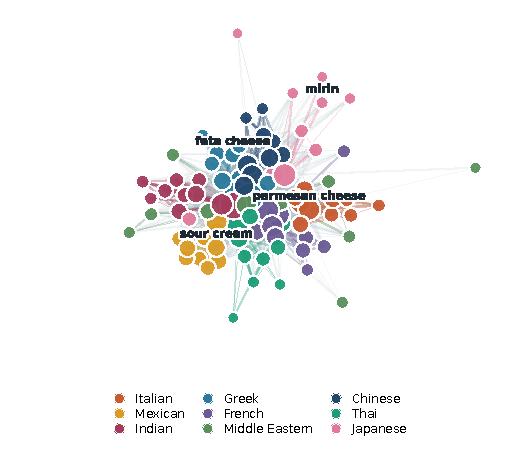
\includegraphics[width=8.7cm]{figures/ingredient_backbone.pdf}
\caption{The ingredient network, reduced to its strongest links. Each node is an ingredient: the ten most distinctive of each cuisine and a few very common ones, sized by its number of recipes and colored by the cuisine where it is most distinctive. Two ingredients are linked when they share at least 30 recipes and the link passes the disparity filter \cite{serrano2009extracting} ($\alpha < 0.005$), which keeps a link only if it carries a larger share of an ingredient's co-occurrences than it would if they were spread evenly over its neighbors. Positions come from the links alone. Ingredients of the same cuisine end up together: 21\% of the links join two nodes of the same color, against 10\% (at most 12\%) in 2,000 shuffles of the colors.}
\label{fig:network}
\end{figure}

\subsection*{A distinctive pair is not always combined on purpose}
Following Ahn et al. \cite{ahn2011flavor}, we measured how much more often each ingredient pair appears in one cuisine than, on average, in the other eight. Green onion and soy sauce appear together in 24.1\% of Chinese recipes, against 2.9\% on average elsewhere. Feta cheese and olive oil are 20.9 percentage points more common in Greek recipes, and fish sauce and lime juice 16.0 points more common in Thai recipes.

A pair can be distinctive simply because both ingredients are common in the cuisine. To separate \emph{what} from \emph{how}, we took the most distinctive pair of each cuisine as nine examples and compared each with 49 randomized networks (Fig.~\ref{fig:pairs}A). In these networks every recipe keeps its number of ingredients and every ingredient stays as common as before within its cuisine and dish type; only the combinations change. Seven of the nine pairs appeared together more often than the central 95\% of these networks. Mexican recipes combined chili powder and cumin 697 times, almost twice the randomized median of 353: the two are combined on purpose. Italian recipes combined olive oil and parmesan cheese 1,277 times, which is fewer than the randomized median of 1,437: the pair is distinctive of Italian recipes only because each of the two ingredients is common there.

\begin{figure*}[t!]
\centering
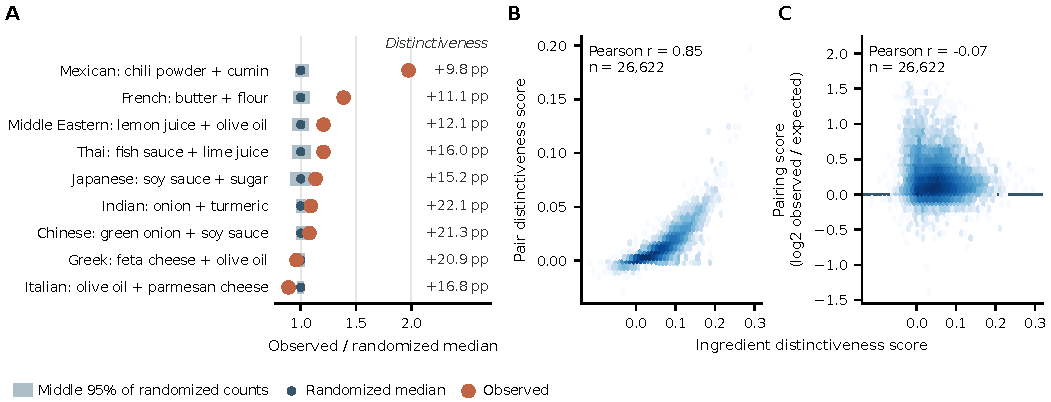
\includegraphics[width=17.8cm]{figures/pairs_and_scores.pdf}
\caption{What a recipe uses and how it combines it are different measurements. (A) For the most distinctive pair of each cuisine, the number of recipes containing both ingredients divided by the median over 49 randomized networks that keep each recipe's number of ingredients and each ingredient's frequency within its cuisine and dish type. The gray interval is the middle 95\% of the randomized counts; the number next to each pair is its distinctiveness in percentage points. Points to the right of the interval are pairs combined more often than their popularity predicts. (B) Ingredient score against pair score for every recipe; darker hexagons contain more recipes. The two are nearly the same measurement. (C) Ingredient score against pairing score: knowing what a recipe uses says almost nothing about how unusually it combines it.}
\label{fig:pairs}
\end{figure*}

\subsection*{What and how are two different scores}
We turned these measures into three scores per recipe. The \emph{ingredient score} is the mean distinctiveness of the recipe's ingredients (\emph{what}). The \emph{pair score} is the mean distinctiveness of its ingredient pairs. The \emph{pairing score} (\emph{how}) repeats the comparison of Fig.~\ref{fig:pairs}A for every pair of the recipe: the number of recipes of the cuisine that contain both ingredients, divided by the number expected in the randomized networks. A pair found twice as often as expected counts $+1$, a pair found as often as expected counts 0, and a pair found half as often counts $-1$ (the $\log_2$ of the ratio), and the score is the mean over the recipe's pairs (Methods). We could score 26,622 of the 26,727 recipes; 105 had fewer than two retained ingredients.

The ingredient and pair scores are strongly correlated ($r=0.85$; Fig.~\ref{fig:pairs}B): a recipe with distinctive pairs is almost always a recipe with distinctive ingredients, so the pair score adds little. The pairing score is different. Its correlation with the ingredient score is $r=-0.07$ (Fig.~\ref{fig:pairs}C) and with the pair score $r=0.06$, so knowing which ingredients a recipe uses says almost nothing about whether it combines them in the usual way. Its highest-scoring pairs are recipe templates: carrot and celery in Italian recipes (the base of a soffritto; 184 recipes against 19 expected), garlic and ginger paste in Indian recipes (76 against 4.0), tequila and triple sec in Mexican recipes (45 against 1.4), and bay leaf and thyme in French recipes (39 against 7.1). Not all templates are traditional: garlic powder with onion powder, or the canned cream soups of Mexican casseroles, also score high.


% TODO: Add review-language results here once that analysis is final.


% Discussion: what the results mean, and their limits. Name our own
% limitations before the reader does. A negative result with convincing
% checks is fine.

\section*{Discussion}

The network gives us a way to describe how characteristic a recipe's ingredient pairs are of its Food.com cuisine tag. It does not tell us whether the dish is culturally authentic. The next step is to compare this score with what reviewers actually say, distinguishing comments that affirm authenticity from those that question it. A review with no mention of authenticity cannot be read as a negative judgment. General sentiment and star ratings should be examined separately.

The two randomizations answer different questions. Shuffling cuisine tags shows that the recipe network is associated with those tags. Preserving ingredient frequencies shows that much of this association can arise because cuisines use different individual ingredients. The smaller remaining difference cannot be attributed uniquely to cuisine-specific pairing rules: recipe families and preparation styles may also contribute. The pair check makes another distinction concrete: olive oil and parmesan are distinctive of Italian-tagged recipes relative to other cuisines, yet occur together less often than the frequency-preserving reference predicts within Italian-tagged recipes. Our recipe pair score measures cross-cuisine prevalence, not a pairing effect independent of ingredient popularity. We will therefore ask whether pair scores add information beyond individual ingredients, while comparing recipes within cuisines and accounting for their review counts and broad dish types. A null result would mean these measurable signatures do not predict how this Food.com audience uses the word ``authentic''; it would not settle the meaning of authenticity more broadly.

Food.com cuisine and course tags are supplied by users, and our manual review found uncertain labels. The ingredient cleaning deliberately merges only clear aliases, leaving some equivalent names separate. Preparation methods, personal memories, and access to ingredients may shape a review but are absent from the pair score. The dataset represents an online recipe community, not all cooking within any of the named cultures. These limits affect both the score and its interpretation alongside review text.


% TODO: Integrate the review-language findings and joint limitations here.


\matmethods{% Methods: enough detail to reproduce every number. This is the argument
% of \matmethods{} in main.tex, so it may contain subsections and equations.

\subsection*{Data}
The Food.com Recipes and Interactions dataset contains 231,637 recipes submitted from 1999 to 2018 and 1,132,367 user reviews \cite{majumder2019generating}. We kept recipes tagged with exactly one of nine cuisines: Italian, Mexican, Indian, French, Greek, Middle Eastern, Chinese, Thai, or Japanese. We mapped regional tags to these groups (for example, \emph{szechuan} to Chinese) and removed 431 recipes tagged with two of the nine. We also removed recipes with fewer than two ingredients and exact duplicates with the same name and ingredient set. Preparation times of zero or above a Tukey fence on $\log_{10}$(minutes) ($k=3$, about 19 hours) were treated as missing. For the review dataset, we removed 12,981 reviews written for community cooking games, 107 replies from recipe authors, and 18 reviews without text. We treated a rating of zero as missing because it likely meant that no stars were given. The processed dataset has 26,727 recipes and 132,744 reviews.

% Network methods used inside the manuscript's \matmethods{...} block.
\subsection*{Ingredient network and recipe scores}
We lowercased ingredient names and merged 72 manually reviewed aliases. We excluded 20 generic names, including salt, pepper, water, and unspecified oil, and names found in fewer than three or more than 35\% of recipes. The resulting binary recipe-by-ingredient matrix has 3,877 ingredient types. An entry of one is a link in the bipartite graph; the ingredient projection joins two ingredients when they appear together in at least one recipe. To describe ingredient concentration across cuisine tags, we calculated each ingredient's entropy over the nine tags, divided by $\log 9$, and averaged across ingredients with their recipe counts as weights. We compared this with 199 shuffles of the recipe cuisine labels on the fixed bipartite network.

For cuisine $c$, let $N_c$ be its number of recipes and $n_{c,ij}$ the number containing both ingredients $i$ and $j$. Following Ahn et al. \cite{ahn2011flavor}, we define the pair contrast as $n_{c,ij}/N_c - \langle n_{d,ij}/N_d\rangle_{d\ne c}$, an equal-weight mean over the other eight cuisines. The pair score for a recipe is the mean contrast over all its retained pairs. To prevent a recipe from increasing its own score, we replace its cuisine term with $(n_{c,ij}-1)/(N_c-1)$ when scoring it. We calculate the ingredient-only score in the same way, replacing pairs with individual ingredients. Recipes with fewer than two retained ingredients have no pair score. For illustrative pair signatures, we require at least 20 recipes containing the pair in the named cuisine; this threshold does not affect recipe scores. We exported both scores with recipe IDs for the later review analysis.

\subsection*{Pairing score}
Within cuisine $c$, let $n_{c,ij}$ be the number of other recipes containing both $i$ and $j$, and $E_{c,ij}$ its mean over 50 Curveball randomizations of the recipe--ingredient matrix within each cuisine (ten attempted trades per recipe), which preserve every recipe's ingredient count and every ingredient's frequency in the cuisine. For leave-one-out, $E_{c,ij}$ is rescaled by $(n_{c,i}-1)(n_{c,j}-1)/(n_{c,i}n_{c,j})$. The pairing lift is $L_{c,ij}=\log_2\left[(n_{c,ij}+k)/(E_{c,ij}+k)\right]$, positive when two ingredients are combined more often than their popularity predicts, and a recipe's pairing score is the mean $L_{c,ij}$ over its retained pairs. This is the network analogue of a collocation score in text. The pseudocount $k$ shrinks rare pairs, for which a count of one or two is mostly chance: 34\% of all recipe pairs have $E_{c,ij}<1$. We chose $k=5$ by split-half reliability: we split each cuisine's recipes at random into two halves, scored every recipe once from each half, and correlated the two scores. The correlation rose from 0.70 with $k=1$ to 0.82 with $k=5$ (Spearman--Brown reliability with all data: 0.82 to 0.90). Scores with $k=2$ and $k=10$ correlate at $r\geq0.98$ with $k=5$, and we report them as robustness checks.

\subsection*{Supporting network comparisons}
We also projected the bipartite graph onto recipes. We measured similarity with $J(r,s)=|I_r\cap I_s|/|I_r\cup I_s|$ and linked recipes sharing at least two retained ingredients with $J\geq0.18$. We kept the union of each recipe's 15 most similar neighbors; link weight was $J$. Cuisine labels played no role in constructing links. Weighted Louvain community detection was run without cuisine labels; we inspected ingredient and title patterns in its largest mixed community. To compare the observed within-cuisine weight share with cuisine sizes alone, we shuffled cuisine labels 199 times over the fixed graph. We then ran 49 Curveball randomizations of the recipe--ingredient matrix within each cuisine, with ten attempted trades per recipe, preserving every recipe's ingredient count and each ingredient's frequency within its cuisine. Another 49 runs restricted trades to recipes of the same cuisine and broad Food.com course type. We rebuilt the recipe projection after every randomization and checked the preserved counts. The first shuffle tests an association between tags and the fixed graph; the ingredient swaps ask how much structure remains after accounting for ingredient frequencies and broad dish types.

For the nine illustrative pairs, we used a separate set of 49 cuisine-by-course-type Curveball randomizations with ten attempted trades per recipe. We counted how many recipes in the named cuisine contained both ingredients in each randomized matrix. We checked that row sizes and ingredient frequencies in every cuisine-by-type group were unchanged after every run. The middle 95\% of randomized counts is a reference range for these nine previously selected pairs, not a confidence interval or a multiple-comparison test.


% TODO: Add text-analysis methods and validation once that analysis is final.
}
\showmatmethods{}

\dataavail{Code, notebooks and the processed datasets are available at \url{https://github.com/EstebanPerez99/cuisine-networks}. The raw data are the Food.com Recipes and Interactions dataset \cite{majumder2019generating}.}

\acknow{We thank the teaching team of 02805 Social Graphs and Interactions.}
\showacknow{}

% Number of references placed in the left column of the last page.
% Adjust once the reference list is final.
\bibsplit[6]

\bibliography{references}

\end{document}
